% 2023本郷祭 マイコン部 部誌 「マイコンHONGOMagazine」 TeXテンプレート

% =環境設定=

\documentclass[b5paper,10pt]{jsarticle}

% 数式
\usepackage{amsmath,amsfonts}
\usepackage{bm}

% 画像
\usepackage[dvipdfmx]{graphicx}

% 段組
\usepackage{multicol}
\setlength{\columnseprule}{0.5pt}

% 表(オリジナルパッケージ)
\usepackage{tabularx}

% 余白
\usepackage[paper=b5j,truedimen,margin=15truemm]{geometry}
\usepackage{ulem}
\usepackage{ascmac}

% ページ番号を削除
\pagestyle{empty}

% ソースコード環境
\usepackage{listings,jvlisting}
\usepackage{listings,jlisting}
\lstset{
  basicstyle={\scriptsize\ttfamily},
  identifierstyle={\scriptsize},
  commentstyle={\smallitshape},
  keywordstyle={\scriptsize\bfseries},
  ndkeywordstyle={\scriptsize},
  stringstyle={\scriptsize\ttfamily},
  frame={tb},
  breaklines=true,
  columns=[l]{fullflexible},
  numbers=left,
  xrightmargin=0zw,
  xleftmargin=0zw,
  numberstyle={\scriptsize},
  stepnumber=1,
  numbersep=1zw,
  lineskip=0.5ex
}
\renewcommand{\lstlistingname}{リスト}

% 書きたい内容に合わせてお好きなパッケージを導入していただいて構いませんが、外部パッケージは提出時に必ず合わせて提出してください。
% また、そのパッケージを使用している部分には必ずコメントをしてください。

% =環境設定ここまで=

\begin{document}

% =タイトル=
\title{書店で見かけたScratchの入門書が簡単すぎるので\\誰からも頼まれていませんが\\勝手にScratchについて解説します。}
\author{TurboWarp狂の副部長}
\date{\today}
\maketitle
% 初めのページのページ番号を削除(\maketitleの影響を回避)
\thispagestyle{empty}

% ここではページごとに段組しています。大きく画像を表示したいときなどは以下を \begin{multicols}{3} 、\end{multicols}のように変更すると文章が終わった直後から空白になります
\begin{multicols*}{3}
  
% 以下本文
皆さんこんにちは。Scratchを(おそらく)極めた、やる気が出ない副部長です。タイトルが一部のああいうラノベのように長いですね。この記事では今後も長ったらしい文、また文法がおかしい文、読みにくい文、「ですます調」と「だである調」が混在する文がずっと登場します。あと紛らわしかったり遠回しな表現もたくさん登場するので、苦手な方、疲れやすい方は次の記事へ進んでくれて構いません。

さて、本題に入ります。いつのことだか忘れましたが、私がUnityとCsharpについて学び始めたころ、それに関する参考書がないかな~と近くの書店のプログラミングコーナーに寄りました。いい感じの解説書は無事手に入りましたが、とある参考書が私の目に留まったんですよね。そう、今回の本題のきっかけ(多少の悪口の対象でもある)となったScratchの参考書です。その場でパラパラとめくってみましたが、簡単。簡単すぎる。読み応え0。さすがに言い過ぎかもしれませんが、私の理想とかけ離れていました。これでは実力のあるScratcher(Scratchをする人)は生まれません。\sout{だから今のScratchは\\民度が低いわけですね。}\\だからScratchが得意という人が少ないんですね。

というわけで前置きが馬鹿みたいに長くなりましたが、今回は通常は参考書で語られない、Scratchの概要とブロックの詳細説明をして行きたいと思います。本当はそれらを使ったプロジェクト作りもやりたかったのですが、如何せん時間の都合上執筆が間に合いそうにないので概要とブロックの説明のみになります。あ、でも私はマイコン部の展示場所にいる(はず)ので来ていただいて質問してくださればちゃんと答えますのでどうぞよろしく。それでは皆さんの待ちに待った目次をどうぞ。

\begin{itembox}{目次}
{1. }scratchの基礎知識\\
{ a. }概要\\
{ b. }Scratchの機能・ブロック\\
{ c. }外部MODのTurbowarp\\
{2. }制作\\
{ a. }使用例\\
{ b. }作品例\\
{ c. }Turbowarpの素晴らしいところ
\end{itembox}

\section{Scratchの基礎知識}
\subsection{概要}
まずScratchとはいったい何なのか。まあこのような説明が必要な方は基礎を一から学ばれた方がよろしいと思うので、ぜひ書店に足を運ぶなり、ネットで記事を読むなりしたほうが分かりやすく学べると思いますが、この章ではそんな時間や余裕のない方のために、簡単に説明をしていこうと思います。

Scratchは一種のプログラミング言語であり、その非常にわかりやすいUI、手軽な操作により様々な教育現場で使われています。あいにく本郷では講座はありません。Scratchの仕組みとしては、「スプライト」と呼ばれる2Dのオブジェクトを編集しステージ上で動かすというのがメインです。エディター画面(図1)にて、左側のパレットからブロックをドラッグ&ドロップしてスクリプトを組み立てていったり、「コスチューム」とよばれるスプライトのスキンを編集したりするといった感じです。
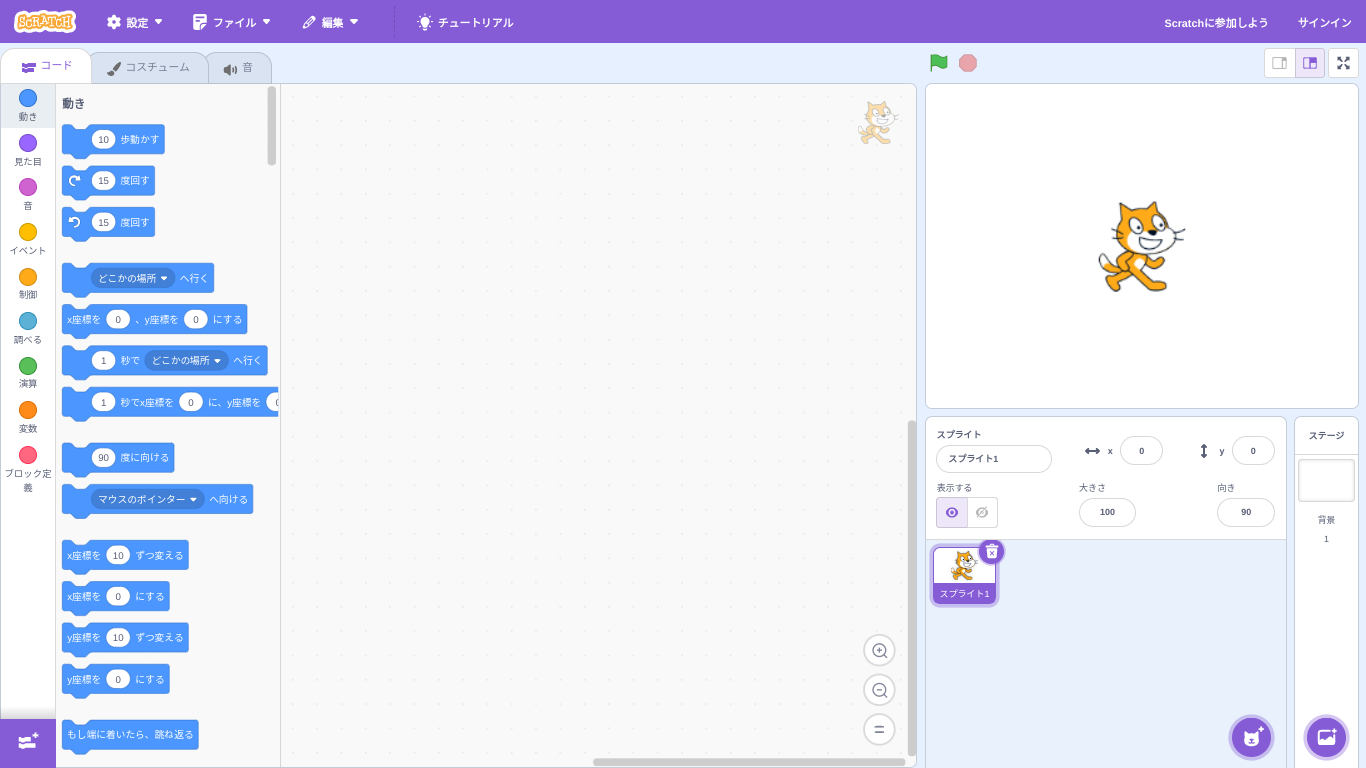
\includegraphics[width=4cm]{editor.png}図1\\
組み立てたスクリプトは、クリックするか、「旗が押されたとき」というイベントカテゴリ(後述)のブロックを先頭にくっつけてステージの上の緑色の旗を押すと実行されます。
少し細かい話をしますと、ScratchはJavaScriptで記述されており、30fpsで動きます。また、拡張機能を使うとLEGOと連動したり、カメラで動きを検知したりすることもできます。

まあ、こんな感じでScratchはキーボードがなくてもマウスだけでプログラミングができるという破格の性能(無料だけど)をしています。
\subsection{TurboWarpとは}
ここからは布教活動となりますので、興味のない方は飛ばしてもらって結構です。

それではまず皆さん唱えましょう。
% ソースコードを見ているあなたも唱えましょう。
TurboWarp(ターボワープ)は神です。

TurboWarpはGarboMuffin氏によって製作されたScrtachのModです。UI、操作方法、仕組みなどはほぼ同じですが、TurboWarpはプロジェクトの軽量化に加え、フリーズ・クラッシュ防止のWarpタイマー、FPSの変更、Scratchにおけるさまざまな制限を解除できる設定など、Scratchと比べて機能が非常に充実しています。さらに、アドオンの設定では、一時停止ボタン、変数マネージャー、ブロックのドロップダウン検索などと地味ですがとてもうれしいっ機能も盛りだくさんです。
また、最近知ったのがTurboWarpの独自の拡張機能(紛らわしいですがアドオンとは別物です)ですが、異常なほど多く、Scratchに既にあるアナログな拡張機能に加え、
Gamepad(ゲームコントローラを連携できる)、
Files(ファイルのインポート・エクスポートができるブロックを追加)、
Runtime Option(通常は自分でいじる必要のある環境設定をスクリプトから調整することが可能)、
Sensing+やClone+やLook+(「調べる」や「見た目」というカテゴリとクローン関連のブロックを追加)、
Clipping&Blending(画像の切り抜きや描写に関する調整が可能)、
Local Storage(ほぼCookie)などと言い足りませんが様々なものがあります。
ちなみに執筆時点でおよそ80個で、まだまだ増えています。
そして、それらのほとんどはまさに「痒い所に手が届く」な便利な機能です。まだScratchをお使いの方はぜひTurboWarpへの乗り換えをご検討ください。

\section{Scratchのブロック}

さて、お次はScratchのブロックについてみていきましょう。先ほどお伝えした通り、Scratchはブロックをドラッグ&ドロップしてスクリプトを組み立てていくのですが、参考書にはブロックに対する説明がありませんでした。これは減点ですね。ということでここからScratchのすべてのブロックとそのカテゴリに対して説明していこうと思います。色々無駄な文が混じっていますがご了承しやがれください。それでは、\\
 _______\\
/│  Hmcc │\\
││ (* '▽') │\\
││  舞昆布 │\\
 ̄ ̄ ̄ ̄ ̄ ̄ ̄ ̄\\
ゆっくりしていってね!!
\pagebreak
\subsection{動き}
動きカテゴリは主にそのスプライトの座標、角度について制御するブロックの集まりです。基本的で直感的に理解しやすいブロックだらけです。

\begin{itembox}{1}
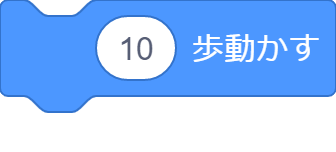
\includegraphics[height=8mm]{images/motion_1.png}
\end{itembox}
使用頻度×\\
そのスプライトが現在向いている方向に向かって座標をxだけずらす。たとえば、スプライトの向き=30°、n=2のとき、このブロックを実行するとx座標が√3、y座標が1変わる。ぶっちゃけ使わない。
\begin{itembox}{2}
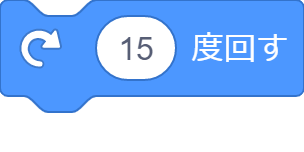
\includegraphics[height=8mm]{images/motion_2.png}

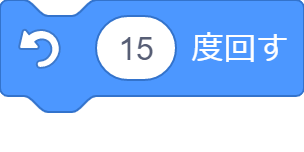
\includegraphics[height=8mm]{images/motion_3.png}
\end{itembox}
使用頻度○\\
そのスプライトの現在の向きをnだけ変える。デフォルトで90°。また、時計回りとその逆で2つブロックがありるが、負の値もちゃんと読み取ってくれて動作するのでただただ無駄なだけ。なんで2個もあるんだ?
\begin{itembox}{3}
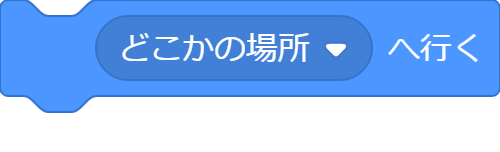
\includegraphics[height=8mm]{images/motion_4.png}
\end{itembox}
使用頻度×\\
このブロックを実行することで、ランダムな場所に行ったりほかのスプライトやマウスに座標を合わせることができる。代用できるので使わない。
\begin{itembox}{4}
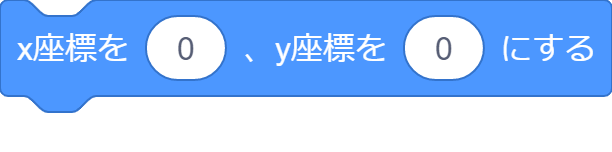
\includegraphics[height=8mm]{images/motion_5.png}
\end{itembox}
使用頻度△\\
xとy座標を変更できるブロック。個別に変更できるほかのブロックがあるので正直いらない。唯一使えるのはxとy座標を同一フレームに変更しなければならない場合(例えばxとy座標がそれぞれに影響される時)。あと個人的にキモい。
\begin{itembox}{5}
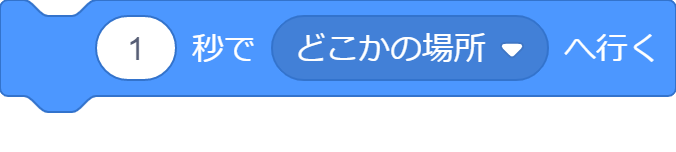
\includegraphics[height=8mm]{images/motion_6.png}
\end{itembox}
使用頻度×\\
「どこかの場所へ行く」の秒数がついたバージョン。座標で事足りるっつってんだろうが。
\begin{itembox}{6}
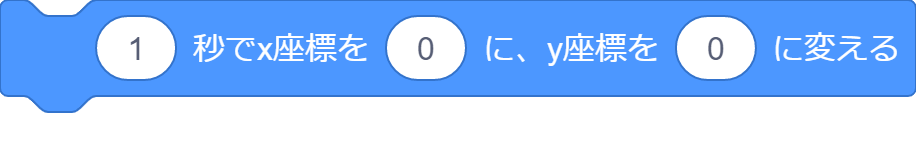
\includegraphics[width=39mm]{images/motion_7.png}
\end{itembox}
使用頻度△\\
少しまともなやつ。FPSに影響されないので、ラグいプロジェクトやTurboWarpでFPSを変更したプロジェクトで使えるかも。基本代替可。あとキモい
\begin{itembox}{7}
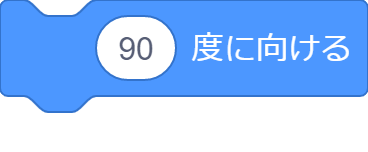
\includegraphics[height=8mm]{images/motion_8.png}
\end{itembox}
使用頻度○\\
スプライトの向きを指定する。使うときはめちゃくちゃ重宝する。自分は最近使っていない。
\begin{itembox}{8}
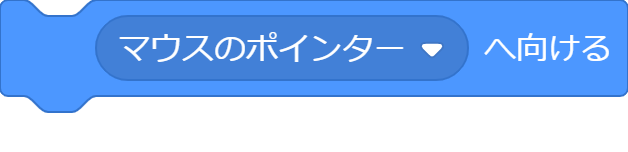
\includegraphics[height=8mm]{images/motion_9.png}
\end{itembox}
使用頻度×\\
座標&三角関数で物足りる。はい。
\begin{itembox}{9}
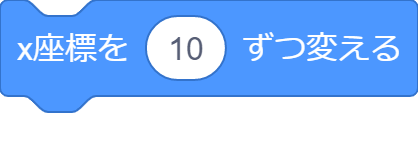
\includegraphics[height=8mm]{images/motion_10.png}

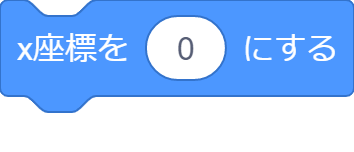
\includegraphics[height=8mm]{images/motion_11.png}
\end{itembox}
使用頻度◎\\
プライトのxy座標の移動は主にこれを使う。これらのブロックのせいでほかのいくつものブロックが死んだ。とても優秀
\begin{itembox}{10}
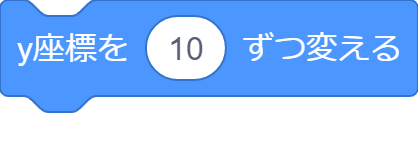
\includegraphics[height=8mm]{images/motion_12.png}

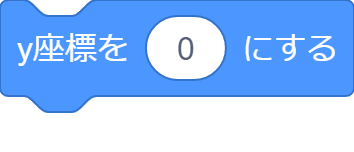
\includegraphics[height=8mm]{images/motion_13.png}
\end{itembox}
使用頻度◎\\
スプライトの座標の指定。位置の初期化、指定場所への移動などはこれを使う。めちゃくちゃ優秀。
\begin{itembox}{11}

\includegraphics[height=8mm]{images/motion_14.png}
\end{itembox}
使用頻度×\\
謎ブロック。実行された時点でステージの端にぶつかったとき、ぶつかった場所に応じてx軸またはy軸で向きを反転する。ほんとに謎。
\begin{itembox}{12}
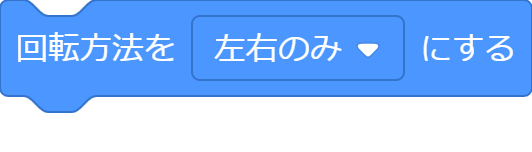
\includegraphics[height=8mm]{images/motion_15.png}
\end{itembox}
使用頻度△\\
左右のみ、回転しない、自由に回転の3つから選べる。左右のみの場合、0°~179°はそのまま、180°(-180°)~359°(-1°)はコスチュームの左右が反転した状態解いて反映される。それ以外の2つは字面通り。
\begin{itembox}{13}
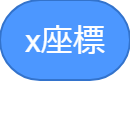
\includegraphics[height=8mm]{images/motion_16.png}

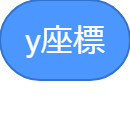
\includegraphics[height=8mm]{images/motion_17.png}
\end{itembox}
使用頻度◎\\
このスプライトの現在の座標を出力する引数。他スプライトの座標を取得するときは調べるカテゴリのブロックが使えるが、正直これで代用できる
\begin{itembox}{14}

\includegraphics[height=8mm]{images/motion_18.png}
\end{itembox}
使用頻度△\\
このスプライトの向きを出力。正直変数を作ったほうが管理しやすい。

\subsection{見た目}
見た目カテゴリは、コスチュームの描写、レイヤー、大きさに関連したブロックと、一部の「なぜここに分類したのかブロック」を含みます。横・縦のみの伸縮ができるブロックをずっと求めていましたが、そんな拡張機能が最近TurboWarpに追加されました。控えめにいって神ですね。

\begin{itembox}{1}
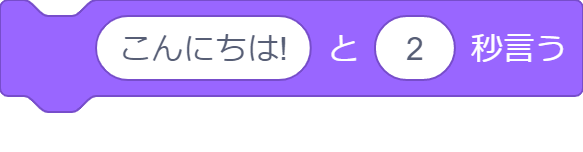
\includegraphics[height=8mm]{images/looks_1.png}
\end{itembox}
使用頻度×\\
こんなブロック、このカテゴリに入れちゃっていいんですか?
\begin{itembox}{2}
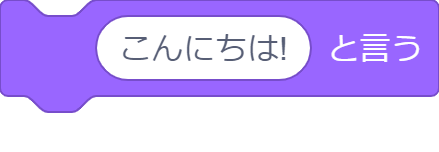
\includegraphics[height=8mm]{images/looks_2.png}
\end{itembox}
使用頻度×\\
本当にこのカテゴリに入れちゃっていいんですか??
\begin{itembox}{3}
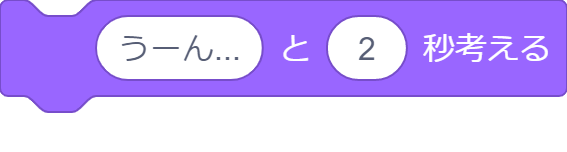
\includegraphics[height=8mm]{images/looks_3.png}
\end{itembox}
使用頻度×\\
運営さん、このブロックはこのカテゴリに属していると思っているんですか???
\begin{itembox}{4}
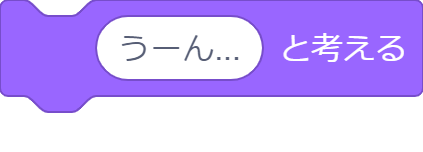
\includegraphics[height=8mm]{images/looks_4.png}
\end{itembox}
使用頻度×\\
まじめな話をすると、一応リアルタイムで何かの値をモニターすることはできます。代替可なのでほぼ意味なし。枠のデザイン変更出来たらまだ使い道はあったんですけどね。ちなみにTurboWarpの拡張機能に、これのほぼ上位互換であるAnimated Textなるものがございまして...
\begin{itembox}{5}
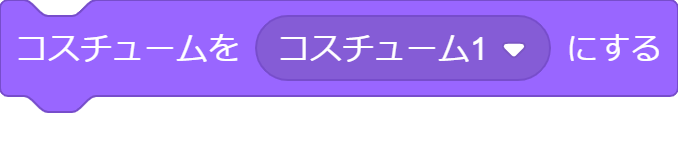
\includegraphics[height=8mm]{images/looks_5.png}
\end{itembox}
使用頻度◎\\
スプライトのコスチュームを変更するときに欠かせない。
\begin{itembox}{6}
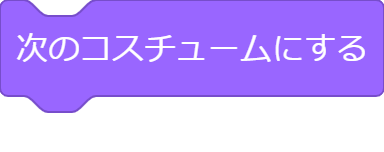
\includegraphics[height=8mm]{images/looks_6.png}
\end{itembox}
使用頻度○\\
「前のコスチュームにする」ブロックもください。そうしたらもっと使ってやりますよ。
\begin{itembox}{7}
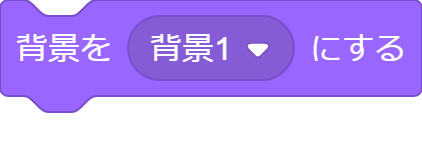
\includegraphics[height=8mm]{images/looks_7.png}

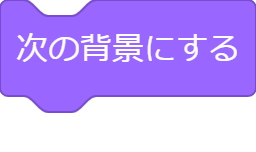
\includegraphics[height=8mm]{images/looks_8.png}
\end{itembox}
使用頻度×\\
背景はステージのスキンを指します。そもそもステージを背景目的で使うことなんてめったにないのでお役御免です。
\begin{itembox}{8}
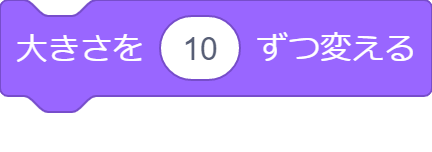
\includegraphics[height=8mm]{images/looks_9.png}

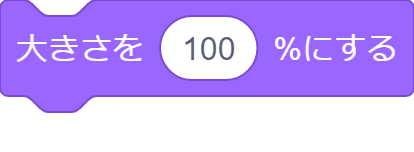
\includegraphics[height=8mm]{images/looks_10.png}
\end{itembox}
使用頻度◎\\
スプライトの大きさを制御できる唯一のブロック。10000%とかにすると当たり判定がおかしくなることがあるので要注意。
\begin{itembox}{9}
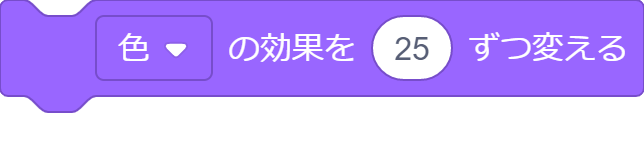
\includegraphics[height=8mm]{images/looks_11.png}

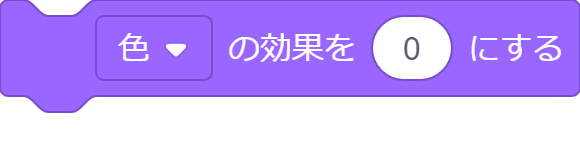
\includegraphics[height=8mm]{images/looks_12.png}
\end{itembox}
使用頻度○\\
ドロップダウンメニューから選んだ画像効果をかける。色、明るさ、透明度などよく見る効果や渦巻、魚眼レンズなど使い道がよくわからない効果がたくさんある。
\begin{itembox}{10}
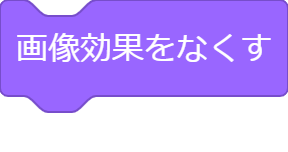
\includegraphics[height=8mm]{images/looks_13.png}
\end{itembox}
使用頻度○\\
一個上のブロックでかけた画像効果をすべて解除。効果をかけまくって何が何だか分からなくなったときに使う。
\begin{itembox}{11}
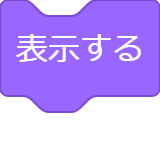
\includegraphics[height=8mm]{images/looks_14.png}


\includegraphics[height=8mm]{images/looks_15.png}
\end{itembox}
使用頻度◎\\
スプライトを表示・非表示にしてくれる。見えてほしくないスプライトはこれで隠しましょう。
\begin{itembox}{12}
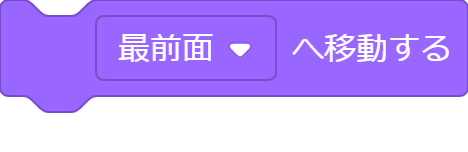
\includegraphics[height=8mm]{images/looks_16.png}

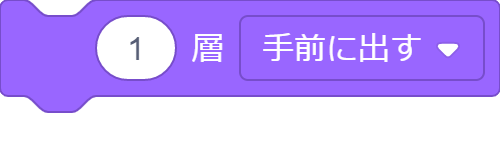
\includegraphics[height=8mm]{images/looks_17.png}
\end{itembox}
使用頻度○\\
Scratchにはレイヤーの概念が存在しており、レイヤーidが大きい方が前面に表示されます。また、1レイヤーにつき1スプライトまでしか配置できません。レイヤーの調節に関しては、TurboWarpの拡張機能「Looks+」を使うことをお勧めします。
\begin{itembox}{13}
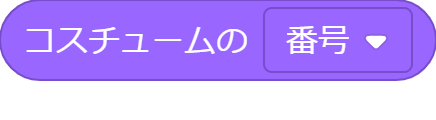
\includegraphics[height=8mm]{images/looks_18.png}
\end{itembox}
使用頻度○\\
ドロップダウンメニューから読み取るものを番号か名前か選択できます。このブロックのおかげでコスチューム名をデータを入れる場所として使うことができます。これは余談ですが、ScratchはコードではaとAを区別できないのに、コスチューム名では区別できます。
\begin{itembox}{14}
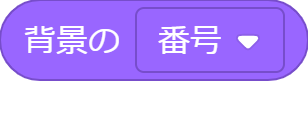
\includegraphics[height=8mm]{images/looks_19.png}
\end{itembox}
使用頻度×\\
いうまでもないですね。もはやスペースの無駄
\begin{itembox}{15}
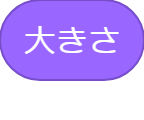
\includegraphics[height=8mm]{images/looks_20.png}
\end{itembox}
使用頻度△\\
(向き)同様変数を作った方が管理しやすいのであまり使わない。

\subsection{音}
音カテゴリはそのまま音に関するブロックの集まりです。特にこれ以上言うことはないですね。
\begin{itembox}{1}

\includegraphics[height=8mm]{images/sound_1.png}
\end{itembox}
使用頻度○\\
音が鳴り終わるまで処理が終わらないので、特に音楽(bgm)を流すときは「ずっと」ブロックと相性がいいので重宝する。
\begin{itembox}{2}

\includegraphics[height=8mm]{images/sound_2.png}
\end{itembox}
使用頻度○\\
音を垂れ流したまま次のブロックが処理される。おもに短い効果音などそのまま垂れ流されても困らない場合、または次のブロックが重要で迅速に処理されるべき場合に使う。
\begin{itembox}{3}

\includegraphics[height=8mm]{images/sound_3.png}
\end{itembox}
使用頻度○\\
ほかのスプライトが鳴らしている音もすべて止めるので要注意。
\begin{itembox}{4}

\includegraphics[height=8mm]{images/sound_4.png}

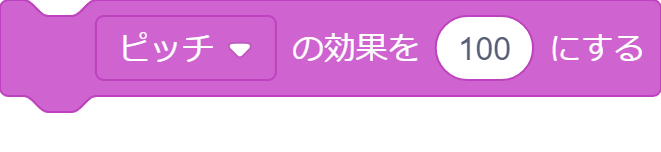
\includegraphics[height=8mm]{images/sound_5.png}
\end{itembox}
使用頻度○\\
ドロップダウンメニューからピッチ、「左右にパン」を選択可能。0でデフォルト。ちなみにピッチを120に設定することでおよそ2倍速、70でおよそ1.5倍速。また-infinityに設定することで(TurboWarpの高度な設定でその他の制限を解除する必要があり)音を一時停止することもできます。Scratchは無理なのでぜひTurboWarpを。
\begin{itembox}{5}
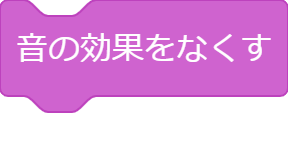
\includegraphics[height=8mm]{images/sound_6.png}
\end{itembox}
使用頻度△\\
「画像効果をなくす」の音版。ピッチのリセットは自分で0に設定したほうがなんとなくすっきりするのであまり使わない。
\begin{itembox}{6}

\includegraphics[height=8mm]{images/sound_7.png}


\includegraphics[height=8mm]{images/sound_8.png}
\end{itembox}
使用頻度△\\
音量はスプライトごとに違うので注意。
\begin{itembox}{7}

\includegraphics[height=8mm]{images/sound_9.png}
\end{itembox}
使用頻度△\\
(向き)と(大きさ)と同じなので割愛。

\subsection{イベント}
さあやってきました、Scratchにて最も重要といえるかもしれないイベンカテゴリです。イベントカテゴリでは、例えば「緑の旗が押された」とか、「メッセージを受け取った」などのイベントをトリガーに、その後ろにくっついているブロックを活性化させます。このカテゴリがなきゃScratchは動きません。なぜなら先頭にイベントカテゴリンのブロックがついていないスクリプトは自動的に動作しないからですね。

ちなみに画像では先頭に猫がくっついておりますがこれはScratchのイースターエッグをTurboWarpの拡張機能で常時onにしているだけで、機能性には全く影響しないので無視してもらって大丈夫です。え?見切れているって?それはTurboWarp側でブロックの画像を出力する際の問題なのでどうしようもないです。ちなみに以降も同じ現象が続くのでご了承ください。私には無理でした。

\begin{itembox}{1}

\includegraphics[height=8mm]{images/events_1.png}
\end{itembox}
使用頻度 ほぼ必須◎◎\\
これがなきゃScratchは始まらない!ぐらいに重要で初心者のころからずっと使っているであろうブロック。今更解説する必要などないでしょう。
\begin{itembox}{2}
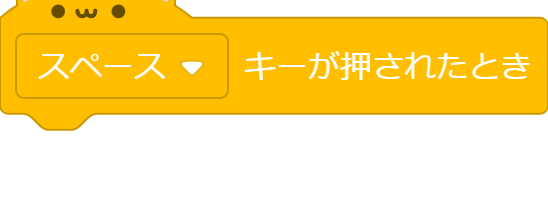
\includegraphics[height=8mm]{images/events_2.png}
\end{itembox}
使用頻度○\\
おそらくあなたも初心者のころに使ったであろうブロック。ほかの条件と組み合わせる場合<(スペース▽)キーが押された>で事足りますが、イベントとして使うときはやはりこのブロックがしっくりきます。ちなみにTurboWarpのアドオンで「キー入力オプションの追加」をONにすることで、ctrlやshift、Enterや記号キーを感知できるようになります。
\begin{itembox}{3}
\includegraphics[height=8mm]{images/events_3.png}
\end{itembox}
使用頻度△\\
「押されたとき」という条件はめちゃくちゃ使うんですけどこれじゃあほかの条件(例えば変数が特定の値の時のみ)とうまく組み合わせることができないんですよね。なので基本的には<<マウスが押された>かつ<(マウスのポインター▽)に触れた>>で代用することになります。
\begin{itembox}{4}
\includegraphics[height=8mm]{images/events_4.png}
\end{itembox}
使用頻度×\\
背景は使わない。
\begin{itembox}{5}
\includegraphics[height=8mm]{images/events_5.png}
\end{itembox}
使用頻度○\\
ドロップダウンメニューから音量かタイマーか選べる。一部のイベントブロック(例えばこれ)は、コードペイン(コードを組む場所)に出しただけで常時プログラムが走っている状態になります。赤丸を押しても止まりません。しかし、条件を満たさない限りは実際にはただの見た目の問題なので気にしないでください。ちなみに小技として、タイマー>0を利用すると、実質的に「赤丸が押されたとき」というブロックを再現することができます。知らない人はぜひチャレンジしてみてください。
\begin{itembox}{6}
\includegraphics[height=8mm]{images/events_6.png}
\end{itembox}
使用頻度◎\\
メッセージは主にスプライト間でのタイミングのやり取りに使われます。普通に便利
\begin{itembox}{7}
\includegraphics[height=8mm]{images/events_7.png}

\includegraphics[height=8mm]{images/events_8.png}
\end{itembox}
使用頻度◎\\
便利。「送って待つ」のほうは、メッセージを受け取ったスプライトが処理を完了するまで次のブロックに進めないので、受け取るスプライトに先に必要な処理をさせる場合に使える。有能。

\subsection{制御}
やってまいりました。イベントカテゴリと並ぶほど重要なやつ、それが制御カテゴリです。これを自由自在に使いこなせれるのが中級者(と勝手に思っています)ので、頑張ってマスターしましょう。

\begin{itembox}{1}
\includegraphics[height=8mm]{images/control_1.png}
\end{itembox}
使用頻度◎\\
初心者の頃は特にお世話になったブロックの一つ。タイミングの調整にめちゃくちゃ使えます。豆知識ですが、正確な秒数はn=1で約1.020秒(パフォーマンスにもよりますが私の場合は1.017~1.023秒でした)、n=0で約0.033秒(=30fpsのときの1フレーム)です。
ちなみに何も入力しなくてもn=0として認識されます。
\begin{itembox}{2}
\includegraphics[height=15mm]{images/control_2.png}
\end{itembox}
使用頻度 ほぼ必須◎◎\\
もはや解説などいりませんね。こんな使いやすいブロック。ちなみに小技ですが、「このクローンを削除する」を「1回繰り返す」で挟むとスクリプトの途中でクローンを全消ししてメインのスプライトだけ処理を継続することもできちゃいます。
\begin{itembox}{3}
\includegraphics[height=14mm]{images/control_3.png}
\end{itembox}
使用頻度 ほぼ必須◎◎\\
ずっと繰り返したい処理に対して使う。条件付きの場合は中にほかのブロックを挟むといい
\begin{itembox}{4}
\includegraphics[height=15mm]{images/control_4.png}
\end{itembox}
使用頻度 ほぼ必須◎◎\\
条件分岐第一弾。if-。特定の条件を満たしたときのみこのブロックで囲んだブロックを処理する。
\begin{itembox}{5}
\includegraphics[height=22mm]{images/control_5.png}
\end{itembox}
使用頻度 ほぼ必須◎◎\\
条件分岐第二弾。if-else-。重ね掛け(elseの部分にまたif-else-を入れる繰り返し)すると見た目が悪くなるが機能性は素晴らしい。
\begin{itembox}{6}
\includegraphics[height=8mm]{images/control_6.png}
\end{itembox}
使用頻度◎\\
何かの条件がそろうまで次の処理に移らない。タイミング合わせや、「ずっと{}」とくみあわせて何かの条件があるときは実行しないようにするのが基本的な使い方かと。
\begin{itembox}{7}
\includegraphics[height=8mm]{images/control_7.png}
\end{itembox}
使用頻度◎\\
「<true?>まで待つ」で待っている間に何か処理をしたい場合に使う。便利。
\begin{itembox}{8}
\includegraphics[height=8mm]{images/control_8.png}
\end{itembox}
使用頻度○\\
ドロメニュから「すべてを止める」「このスクリプトを止める」「このスプライトのほかのスクリプトを止める」が選択可能。すべてを止めると文字通りプロジェクトのすべてが止まるのでほぼ使わない。このスクリプトを止めるは条件分岐にはめ込むのが基本の使い方。スプライトのほかのスクリプトは現在実行している塊以外のスプライト内のスクリプトをすべて止める。「ずっと{}」も止められてしまうので要注意。
\begin{itembox}{9}
\includegraphics[height=8mm]{images/control_9.png}
\end{itembox}
使用頻度◎\\
なんでイベントカテゴリじゃないんですか。メインスプライトでは絶対に動作することのないイベントブロックです。クローンされたときの初期化をさせたり、うしろに「ずっと{}」をつけて削除されるまで所定の処理を行わせるのが一般。
\begin{itembox}{10}
\includegraphics[height=8mm]{images/control_10.png}
\end{itembox}
使用頻度◎\\
変数などのパラメーターや現在のコスチュームや座標などが全く同じクローンを作ります。一般的には識別子として使う変数を1ずつ変えながら「(n)回繰り返す」にはめ込んで使う。実行者がクローンでもクローンを作れます。
\begin{itembox}{11}
\includegraphics[height=8mm]{images/control_11.png}
\end{itembox}
使用頻度◎\\
クローンは作ったら必ずいつかは消去しなければクローン上限数(300体)に達して死ぬので必須です(TurboWarpの高度な設定で上限をなくせますが重いです)。さっきも書きましたが「(1)回繰り返す」で挟むとクローンを全消ししてメインスプライトだけ残せます。

\subsection{調べる}
このカテゴリはその名の通りデータを取得したり真偽値を出したりするのが主な目的です。これまで紹介してきたブロックの(n)や<true?>のところにはめ込んで使います。

\begin{itembox}{1}
\includegraphics[width=39mm]{images/sensing_1.png}
\end{itembox}
使用頻度◎\\
スプライトがマウスに触れたらtrueを返します。そのまま使ってもいいし、のちに紹介する<マウスが押された>と< <true?>かつ<true?> >で結ぶことによってイベントカテゴリのあのブロックを代替することができます。
\begin{itembox}{2}
\includegraphics[height=8mm]{images/sensing_2.png}
\end{itembox}
使用頻度×\\
スプライトが指定した色に触れるとtrue。そんなあいまいな判定方法じゃあだめですよ。
\begin{itembox}{3}
\includegraphics[height=8mm]{images/sensing_3.png}
\end{itembox}
使用頻度×\\
ちなみに、コスチュームがpngでもsvgでも問題なく反応する。透明は白として扱うので注意
\begin{itembox}{4}
\includegraphics[height=8mm]{images/sensing_4.png}
\end{itembox}
使用頻度○\\
コスチュームの形やサイズが変なせいで<(マウスのポインター▽)に触れた>が変な挙動をするときに試してみよう。安定します。
\begin{itembox}{5}
\includegraphics[height=8mm]{images/sensing_5.png}

\includegraphics[height=8mm]{images/sensing_6.png}
\end{itembox}
使用頻度○\\
プレイヤー側からデータをインプットできる貴重な手段です。実行すると入力欄が出てきて、入力し終えて確定するまで次のブロックが処理されません。入力した内容は(答え)から取り出せます。もう一回質問すると(答え)は上書きされて内容がないようですになってしまうので、その前に変数に保存しておきましょう。余談ですが、スプライトが「表示」ブロックによって見えていれば、スプライトから吹き出しが出てきます。例の見た目カテゴリのジャンルが間違ってるブロックと同じ挙動ですね。また、スプライトが「隠す」ブロックによって隠れていると、入力欄の上に直接文章(ここではquestion)が出てきます。
\begin{itembox}{6}
\includegraphics[height=8mm]{images/sensing_7.png}
\end{itembox}
使用頻度◎\\
「[スペース▽]キーが押されたとき」の真偽値バージョン。ほかの条件と併用できるので便利。同じくTurboWarpでアドオンでONにすればctrlやshiftなどいろいろなキーが検知できる。あなたも是非TurboWarpを使ってみませんか?
\begin{itembox}{7}
\includegraphics[height=8mm]{images/sensing_8.png}

\includegraphics[height=8mm]{images/sensing_9.png}

\includegraphics[height=8mm]{images/sensing_10.png}
\end{itembox}
使用頻度◎\\
マウス関連。これらを使ってマウスを感知したりする。また、使うところはあまりないが、1f前のマウスの座標と比べることでマウスの速さがわかったりする。
\begin{itembox}{8}
\includegraphics[height=8mm]{images/sensing_11.png}
\end{itembox}
使用頻度×\\
ゲーム画面から直接マウスでドラッグできるようにするというものなのだが、条件での制御がめんどくさいので、こんなの使うくらいだったらマウスの座標を使って自作したほうが早いし便利である。
\begin{itembox}{9}
\includegraphics[height=8mm]{images/sensing_12.png}
\end{itembox}
使用頻度×\\
音カテゴリの(音量)とは違って、こちらはあなたのデバイスに内蔵されているマイクから取得した音量です。つまりリアルワールドでの音量です。使わん。
\begin{itembox}{10}
\includegraphics[height=8mm]{images/sensing_13.png}

\includegraphics[height=8mm]{images/sensing_14.png}
\end{itembox}
使用頻度◎\\
FPSやラグに影響されない正確なタイマー。フレーム単位で重要なことをしたいとき、ただ単にタイマーとして使うときなどと使い道盛りだくさん。裏技もいくつかある。自分で探してね。
\begin{itembox}{11}
\includegraphics[height=8mm]{images/sensing_15.png}
\end{itembox}
使用頻度○\\
ほかのスプライトのデータを取得できる。具体的には座標、コスチューム番号、その酢スプライト固有の変数の値など。クローンのデータを取得できないのが玉に瑕。
\begin{itembox}{12}
\includegraphics[height=8mm]{images/sensing_16.png}

\includegraphics[height=8mm]{images/sensing_17.png}
\end{itembox}
使用頻度△\\
前者は現在の年、月、日、曜日、時、分、秒が取得できる。後者は字面通りそのまま。乱数生成に使えるかも?
\begin{itembox}{13}
\includegraphics[height=8mm]{images/sensing_18.png}
\end{itembox}
使用頻度○\\
Scratchでは結構使う。プレイヤーのアカウント名を取得できるので、たとえばRPGゲームのセリフに差し込んだり、セーブコードに混ぜてその人以外プレイできないコードを作ったりできる。アカウントにサインインしていない状態で実行すると何もアウトプットしない。ちなみにTurboWarpでは「編集」ボタンで自由に変更できる。

\subsection{演算}
このカテゴリのブロックはずべ手演算関係です。基本全部よく使う。
\begin{itembox}{1}
((n1)+(n2))

((n1)-(n2))

((n1)*(n2))

((n1)/(n2))
\end{itembox}
使用頻度 ほぼ必須◎◎\\
逆に◎じゃない人の理由を知りたい。四則演算なしで数字をどう処理するん?
\begin{itembox}{2}
((n1)から(n2)までの乱数)
\end{itembox}
使用頻度◎\\
最も基本的な乱数生成器。シードに時間を使っているので、異なるスプライト間でも同時に乱数を取得すれば同じ結果になる。そこだけ注意。
\begin{itembox}{3}
<(n1)>(n2)>

<(n1)<(n2)>
\end{itembox}
使用頻度◎\\
これは四則演算に入ります。2個ありますが、私は見た目的にどうしても変数を左において定数を右に置きたいのでどちらも使っています。
\begin{itembox}{4}
<(n1 or text)=(n2 or text)>
\end{itembox}
使用頻度 ほぼ必須◎◎\\
ほかの言語でいう「==」ですね。数字同士でも文字同士でも使えるので何も考えずに使えて便利。ただ、aとAを区別できないのが残念。そういう時はコスチュームの名前を使って判別しましょう。
\begin{itembox}{5}
<<true?>かつ<true?>>

<<true?>または<true?>>

<<true?>ではない>
\end{itembox}
使用頻度ほぼ必須◎◎\\
いわゆる論理ゲートです。それぞれand、or、notに当たります。xorはこれらを使って作れるので問題なし。
\begin{itembox}{6}
((text)と(text))
\end{itembox}
使用頻度◎\\
文字列編集に特化したブロックです。scratchでは変数や特にリストと一緒に使われます。詳しくはリストで解説します。
\begin{itembox}{7}
((text)の(n)番目の文字)
\end{itembox}
使用頻度◎\\
同じく、文字列編集に特化しています。というか、このブロック(とさっきのやつ)がないと文字列の部分的な置き換え・挿入もままなりません。
\begin{itembox}{8}
((text)の長さ)
\end{itembox}
使用頻度◎\\
上記の2ブロックと一緒に使うと幸せになります。
\begin{itembox}{9}
<(text1)に(text2)が含まれる>
\end{itembox}
使用頻度○\\
リストカテゴリにこれのほぼ上位互換があるのであまり使われません。でも使いやすい。
\begin{itembox}{10}
((n1)を(n2)で割った余り)
\end{itembox}
使用頻度△\\
余りなんか求めてどうするん?乱数生成など一部のプログラムでは使えなくもないが、ほとんど2個次のブロックに出番を取られている。
\begin{itembox}{11}
((n1)を四捨五入)
\end{itembox}
使用頻度△\\
極限値など処理が長引く際に短縮するために使うこともあるが基本そんなに出番はない。ちなみに数学的に正しいけれど紛らわしい例として、-1.5は四捨五入したら-1になります。
\begin{itembox}{12}
((n)の[絶対値▽])
\end{itembox}
使用頻度◎\\
四則演算と論理ゲートの次によく使うブロックです。ドロメニュから絶対値、切り上げ&下げ、平方根、三角関数一式、ln、10^、log、e^が選択できます。これはもう使わない理由がないですね。ちなみに切り上げ&下げは四捨五入同様少し紛らわしいところがあるので要注意。三角関数は3Dプロジェクトを作るうえpenと一緒に欠かせません。ちなみに、x^yを計算したいときは( ( ((x)の[ln▽]) * (y) )の[10^▽])で計算できます。\sout{紛らわしかったら自分で\\模索してみてください。}
\subsection{変数}
まあまあ多くの人がつまずくところ、変数です。中級者レベルになるとさすがに使いこなせると思うのですが一応解説します。

変数とはいったい何なのでしょうか。まずは名前から推測してみましょう。変わる数...さっぱり、という方が多いのではないのでしょうか。(まあ実際バンバン値変わりますね。)何も知らない人に推測してもらったところ、「方程式のxとかそういう感じ?」という回答が返ってきました。まあながち間違いではないですね。

きちんと定義すると、変数というのはデータを一時的に保管できるものです。そういわれても分かりにくいでしょうから例を挙げてみます。例えばそこに紙切れがあって、その上にHMCCと書いてあったとしましょう。このとき、変数は紙切れ\underline{そのもの}、そして紙切れに書かれている「HMCC」という文字が変数が保管するデータに当たります。変数というのはデータを保管、つまり記憶しておくための容器、器、受け皿、箱\underline{そのもの}にすぎません。何が入っていようと変数は変数です(ちなみに容器の名前が変数名だったりしますが紛らわしいので一旦忘れてもokです)。\\ 
文章で頭がやられた人はこちらをご覧ください。

「」 ←変数(そう、データを入れる枠そのもの)\\
\\
「HMCC」 ←変数(値を読み取ると``HMCC'')\\
\\
「12*34」 ←変数(値は``12*34'')\\

さあ、変数とはなにか大体イメージがつかめましたか?つかめなかったらマイコン部の敷地にいる私に声をかけてください。完全にわかるまでお付き合いいたします。( -`ω-)

変数の概念がわかったところで、変数の目的に戻ります。(また紙切れの例です)おそらくですがあなたが紙切れに文字を記した目的は、忘れないようにするためか、それかほかの人に伝えるかでしょう。そう、「わすれないように」と「つたえるために」。それこそが(私的には)変数の目的です。プログラムのが出した値(データ)なんてもう一度実行すれば上書きされますよね。しかし出したデータを変数に書き込むことで、プログラムはデータを「覚える」ことができるのです。さらにその変数をほかのプログラムに「渡す」こともできちゃうのです。これが私が把握できている変数の目的です。
\begin{itembox}{1}
[variable▽]を(n)にする
\end{itembox}
使用頻度 ほぼ必須◎◎\\
変数の値を設定する。変数について解説するべきものは冒頭でしちゃったから言うことがほとんどない。
\begin{itembox}{2}
[variable▽]を(n)ずつ変える
\end{itembox}
使用頻度 ほぼ必須◎◎\\
変数の値をnだけ変更する。[variable▽]のところを選択じゃなくて代入可能の(variable▽)にしてほしかったけど最近TurboWarpにそんな拡張機能が追加されたので満足しています。
\begin{itembox}{3}
変数[variable▽]を表示する

変数[variable▽]を隠す
\end{itembox}
使用頻度×\\
変数モニターをステージ上に出す。デフォルトはオレンジ色で確かどうこうするとアクセントカラーが変わると聞いたことはあるもののどっちにしろデザインは変えられずダサいので却下。なお、変数モニター自体はデバッグで便利なので有用。
\begin{itembox}{4}
(variable)
\end{itembox}
使用頻度 ほぼ必須◎◎\\
veriableは英語で変数で、仮の名前。つけようと思えばほぼどんな名前も付けられる。上2個のブロックで代入されたデータを返す。ちなみに、ほかの多くの言語ではstring形式(文字)、int形式(整数)、float形式(実数)の変数がそれぞれあって、違う型のデータは入れられない。しかしScratchはなぜか変数のタイプが一つしかなく、どんな型のデータも入れられる。前までは何も考えずにデータをぶち込めると喜んでいたが、最近初心者にとっては余計デバッグが大変になる要因の一つのではないかと心配している。ちなみに自分はそれで躓いたことはなかった。

Scratchではクラウド変数というものがある。単刀直入に言おう。むずい。仕様がめんどくさい。制限がだるい。

少し読者の皆様は戸惑っているかもしれない。しかしこいつは私にとって多少なりのトラウマである。

少し詳しく話そう。まず、クラウド変数とはなんぞや。クラウド変数というのは、Scratchアカウントを持った人々が同じプロジェクトを開いているとき、Scratchのサーバーを通して共有される変数のことである。つまりオンラインで共有される変数だ。これだけ聞くと便利そうかもしれない。次はクラウド変数の制限について少し見てみよう。\\\\
・作れる上限数10個\\
・0~9までの数字256個までと`.'が一個、`-'が一個までしか使えない。\\\\
お分かりいただけただろうか。伝えられるデータ量が圧倒的に少ないのだ。測ってみたところ、3KBぐらいしかない。これでオンラインゲームを作るのは無理がある。64x40のマスにそれぞれ10色のうちどれかを配置するだけですべて使い切ってしまう。これはさすがに無理のではないのだろうか。

...などとgriffpatch氏の作品を見るまでは思っていた。おそらくあなたも知っているだろう、Scratch界の神。あの方の作品はぜひあなたご自身で見ていただきたい。余談だがpaper minecraftの原版も作ったのはこの方である。

そして、クラウド変数の仕様であるが、こちらは私からしてもかなり意味不明な仕様となっており、説明できる自信がないので、ぜひあなた自身の目で確かめてもらいたい。覚悟しておきましょう。\\
なお、TurboWarpの拡張機能でこれよりよっぽど使いやすい物があるので是非チェック。\\
変数編、終

\subsection{リスト}
続いてのカテゴリはリストです。リストというものは、その名の通り複数の要素が並ぶ配列です。変数と深くかかわっています。

これだけではよく分からないだろうと思うので少し詳しく解説します。リストというのは0個以上の要素(変数として考えてもらってok)の集合体で、必要に応じて要素を作ったり消したり、要素が内蔵するデータを書き換えたりすることができます。そして、リストが含む要素のそれぞれにデータを保管できるので、データのセットを楽に保管することができます。ではなぜリスト、つまり要素の集合体をたくさんの変数としてではなく、わざわざリストとして扱うのでしょうか。それは、変数を何番目かで管理できるからです。例えば、以下のようなマップを1列ずつリストに書き込んだとしましょう。\\
○●○\\
●●○\\
○○●(○は0、●は1)\\
そうすると、リストの内容は[「010」,「110」,「001」]となります。このとき、保存したマップの2行目の3番目の文字を読み取りたいときは、リストの2番目の3文字目を読み取るだけです。なぜならここではリストの要素は行と、要素のデータがそれぞれの行のデータと対応しているからです。少し難しいですが優れている仕組みであるとわかっていただければokです。

では、要素は要素(つまり変数)の集合体なので、リストとそれが含む要素をつかえば変数は要らないのでしょうか。答えは△です。リストの要素は変数として問題なく使えるので、やろうと思えば全然代替できます。しかし、要素をつかうには毎回リストの何番目かを指定しなければならないので、変数に比べて使うのに比べてひと手間かかります。そのため、カウンターといったセットではないデータを管理する際は変数が手軽です。また、リストは変数と組み合わせることでより一層力を発揮することができます。スマホ(変数、使いやすい)とパソコン(リスト、万能)みたいな関係ですね。後どうでもいいですが、長く使っていると要素などというめんどくさい概念は忘れて、代わりにデータがならんいるという風に解釈するようになるのですが、もしかしたらこちらの方が理解しやすい人もいると思うので一応書いておきました。ではブロック紹介をどうぞ。
\begin{itembox}{1}
(data)を[list▽]に追加する
\end{itembox}
使用頻度◎\\
リストの最後尾に要素を追加します。要素になにもデータを持たせたくないときは空欄のままで構いません。
\begin{itembox}{2}
[list▽]の(n)番目を削除する
\end{itembox}
使用頻度◎\\
n番目の要素をデータごと消します。以降のブロックもそうですが、ここのnには「all」だったり「random」だったり一部の文字を入れても機能します。なお、そこに直接文字を打ち込むことはできないため、コピペする形になります。
\begin{itembox}{3}
[list▽]のすべてを削除する
\end{itembox}
使用頻度◎\\
基本初期化でしか使えませんがデータを読み取る際は頻繁に初期化するのでokです。
\begin{itembox}{4}
[list▽]の(n)番目に(data)を挿入する
\end{itembox}
使用頻度◎\\
文字通り挿入します。挿入したデータがn番目となり、もともとn番目以降のデータは1つ下に下がります。
\begin{itembox}{5}
[list▽]の(n)番目を(data)で置き換える
\end{itembox}
使用頻度◎\\
こちらも文字通り置き換えるだけ。置き換え元が存在していない場合(たとえばリストに3つしか要素がないのに4番目を置き換えようとした)は何も起きないので先にほかのブロックで追加しておこう。
\begin{itembox}{6}
([list▽]の(n)番目)
\end{itembox}
使用頻度◎\\
要素のデータを出力する。いちいちリストの何番目か明示しないといけないため、変数として使うのはあまりよろしくない。ちなみに、リストの仕様上要素は削除できるので、これを使えばスクリプトだけで削除も追加もできちゃう模擬変数が作れます。確かこれをリスト変数とかといったはずです。
\begin{itembox}{7}
([list▽]中の(data)の場所)
\end{itembox}
使用頻度◎\\
文字通り。ここで注意したいのが、リストの中に目当てのデータが2つ以上含まれていても、1つ目の場所しか出力しません。え?ちょうどこの仕様で困っているって?TurboWarpを使いましょう(自分でもうるさく感じてきました)。
\begin{itembox}{8}
([list▽]の長さ)
\end{itembox}
使用頻度◎\\
リストが含む要素の数を返す。「(n)回繰り返す{}」と相性がいい。当然だが要素が何のデータも持っていなくてもカウントする。
\begin{itembox}{9}
<[list▽]に(data)が含まれる>
\end{itembox}
使用頻度○\\
「そうか含まれるのか。だからどうした。」的なブロック。使えなくもないがわざわざ使う理由がそんなにない。たまに本領を発揮して無双(?)する。
\begin{itembox}{10}
リスト[list▽]を表示する

リスト[list▽]を隠す
\end{itembox}
使用頻度△\\
変数のアレのリスト版。デバッグではリストもモニターを使う。変数のアレと同じ運命をたどるとおもいきや、Scratchにおいて唯一リストのモニターはコピペできる文字列をスクリーン上に表示できるので使いどころはまだある(セーブコードとか)。しかしきみはTurboWarpの(以下略)
\begin{itembox}{11}
(list)
\end{itembox}
使用頻度△\\
リストの要素を全部ぶわぁああと返す。要素同士をスペースでくっつけて一つにしてくるので少し扱いづらい。なぜなら要素のデータに含まれるスペースと区別がつかないから。(リストの(n)番目)とかで読み取った方が早くて便利。

\subsection{ブロック定義}
この名前から、一部の人には非常に難しいのではないかという印象を抱かれるかもしれません。しかし安心してください。変数やリストに比べてもそんなに難しくありません。なぜなら新しい概念などは登場しないからです(どこからともなく歓声があがる)。初心者だったころの私は、この名前を見て拡張機能的なやつが作れるのか!?とドキドキしていましたが全くそんなことはなかったですね(笑)。正直、全然必須ではなく、あったらうれしいなー程度のものです。しかし、使いこなせるに越したことはないです。
あと、定義ブロックだけは説明がめんどくさいので図を載せていきます。え?なぜ今までのブロックは図がないかって?LATEXに図を挿入するのがめんどくさいからです()。\\

それでは解説をどうぞ。
\begin{itembox}{使用例1}
\includegraphics[width=4cm]{images/teigi_2.png}
\end{itembox}
ブロック定義は、何個かのブロックをつなげてそれを一個のブロックにまとめるという機能です。
名前は自由に設定できるので分かりやすい名前に設定しておきましょう。別にふざけた名前を付けてもいいですヨ。この場合では、\\\\
\includegraphics[width=4cm]{images/teigi_1.png}(見切れてるのはお許しください)
のように変なイベントブロックみたいなやつにブロックをくっつけています。そして、欄中のブロックを実行することで、くっつけたブロックがすべて実行されます。何個かオプションはありますが、基本はたったのこれだけです。ね?簡単でしょ?
\begin{itembox}{使用例2}

\end{itembox}

定義ブロックは、何個かのブロックを圧縮したものとなります。基本的な使い方としては、何回も使うような同じブロックの集合体を定義ブロックとして圧縮して見た目をよくして総ブロック数を抑えます。引数も設定できるので、


% ソースコードを挿入するときは以下のようにしてくださいS
\begin{lstlisting}[caption=Sample]
mes "hello, world!"
\end{lstlisting}

\end{multicols*}
\end{document}
